\documentclass[unknownkeysallowed, 10pt, a4 paper, handout]{beamer}

% Custom beamer theme
\usepackage{../style/beamerthemeCustom}
\newcommand{\HRule}{\rule{\linewidth}{0.5mm}}   %FOR TITLEPAGE

\usepackage{changepage}       % adjustwidth

\setlength\parskip{0.3cm}

\definecolor{darkgreen}{RGB}{0,100,0}
\newcommand{\green}[1]{\textbf{\textcolor{darkgreen}{#1}}}
\newcommand{\red}[1]{\textbf{\textcolor{red}{#1}}}

\newcommand{\focus}[1]{\textbf{\textcolor{red}{#1}}}
\newcommand{\ra}{$\longrightarrow$ }
\newcommand{\lra}{$\longleftrightarrow$ }

\newcommand{\code}[1]{\colorbox{black}{\color{green}\texttt{#1}}}

% Command to create two side-by-side minipages
\newcommand{\sidebyside}[5]{
  \begin{minipage}{#1\textwidth}
    #2
  \end{minipage} #3 \begin{minipage}{#4\textwidth}
    #5
  \end{minipage}
}

\begin{document}

\begin{frame}
  \begin{center}

    \definecolor{myblue}{RGB}{51,51,179}
    \setbeamercolor{block body}{use=structure,fg=white,bg=myblue!20!myblue}

    \begin{block}{}
      \Large
      \centering
      Linux Basics IV:\\
      Basic shell scripting
    \end{block}

    \vspace{6mm}
    \large
    \textsc{Adriano Angelone, Graziano Giuliani} \\

  \end{center}
\end{frame}

\begin{frame}[label=outline]{Course Outline}
  \begin{itemize}
    \item UNIX/Linux Basics
    \item Intermediate shell commands
    \item Editing and compiling source code
    \item Text file manipulation
    \item \focus{Basic shell scripting}
  \end{itemize}

  \vspace{6mm}

  \centering
  Download slides and exercise files with the command\\
  \code{git clone https://github.com/AA24KK/LinuxBasics.git}\\
  \vspace{1mm}
  or download a ZIP archive at
  \vspace{1mm}
  \code{https://github.com/AA24KK/LinuxBasics/archive/master.zip}

  \vspace{2mm}

  Adriano: \focus{aangelon@ictp.it}, Room 263, ICTP\\
  Graziano: \focus{ggiulian@ictp.it}

\end{frame}

\begin{frame}
  \begin{center}
    \frametitle{Why shell scripting}

    Reuse multiple times the same command:\\
    \focus{less work, less bugs}

    What are the basics:
    \begin{itemize}
      \item Variables
      \item Conditionals
      \item Loops
    \end{itemize}
  \end{center}
\end{frame}


\begin{frame}
  \begin{center}
    \frametitle{Variables I}

    Variables contain data\\
    they have a label (\focus{name}) and a \focus{content}

    \begin{center}
      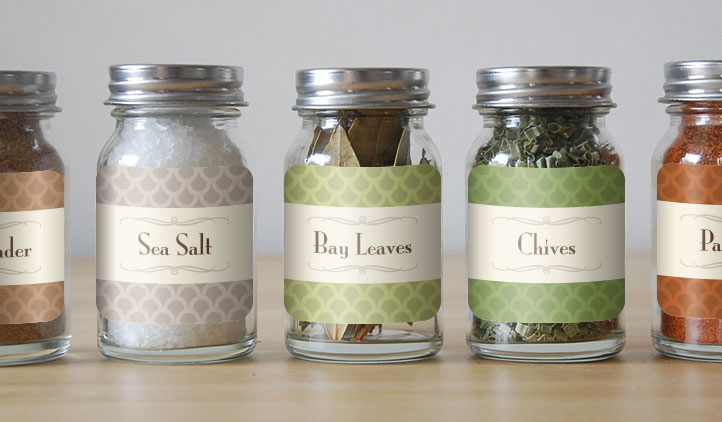
\includegraphics[width=0.72\textwidth]{pics/jars.jpg}
    \end{center}

    In bash, variables \focus{have no type}:\\
    \focus{everything is a string, with arithmetic sometimes possible}
  \end{center}
\end{frame}


\begin{frame}
  \begin{center}
    \frametitle{Variables II}

    Variables are initialized when you use them the first time:\\
    \focus{you can call non-existing variables}, usually trouble\\
    (unless you put \code{set -u} in your script)

    \vspace{5mm}

    \sidebyside{0.50}{
      \centering
      \focus{Assignment}: give a variable a value\\
      \code{<variable name>=<value>}

      \vspace{3mm}

      \focus{Expansion}: access the value\\
      \code{\$<variable name>}
    }{\hfill}{0.45}{
      \begin{center}
        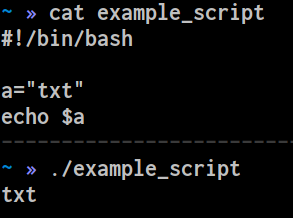
\includegraphics[width=0.70\textwidth]{pics/variables_1.png}
      \end{center}
    }

    \vspace{5mm}

    Usually it's good to use \code{"\$<variable name>"}\\
    to avoid problems if variable contains spaces
  \end{center}
\end{frame}

\begin{frame}
  \begin{center}
    \frametitle{Variables III}

    \sidebyside{0.50}{
      \focus{(Simple) printing}: \code{echo}\\

      \focus{Reading} from standard input: \code{read}
      \code{read -p}: \focus{write prompt}
    }{\hfill}{0.45}{
      \begin{center}
        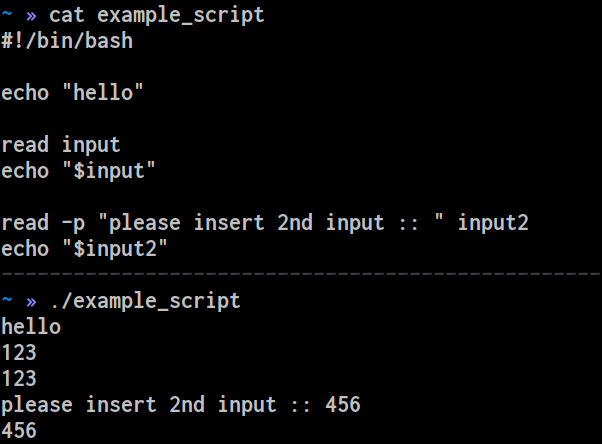
\includegraphics[width=1.00\textwidth]{pics/echoread.png}
      \end{center}
    }

    \vspace{6mm}

    \sidebyside{0.50}{
      \centering
      Easy to make variable values\\
      interact with strings

      \vspace{2mm}

      Use \code{\$\{<variable name>\}}\\
      to avoid expanding another variable
    }{\hfill}{0.45}{
      \begin{center}
        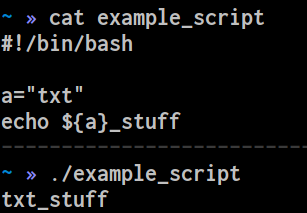
\includegraphics[width=0.70\textwidth]{pics/variables_2.png}
      \end{center}
    }
  \end{center}
\end{frame}


\begin{frame}
  \begin{center}
    \frametitle{Variables IV}

    \sidebyside{0.40}{
      \centering
      \focus{Command substitution}:
      \code{<variable>=\$(<command>)}\\
      outputs command in variable
    }{\hfill}{0.56}{
      \begin{center}
        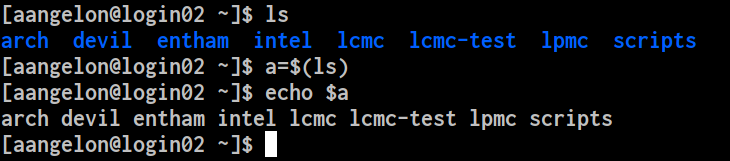
\includegraphics[width=0.90\textwidth]{pics/substitution.png}
      \end{center}
    }

    Some variables are defined system-wide by default: e.g.,

    \vspace{-2mm}

    \begin{itemize}
      \item \code{HOME}: path to your home folder
      \item \code{PATH}: where commands will be searched for if no path specified
    \end{itemize}

    \vspace{-3mm}

    \begin{center}
      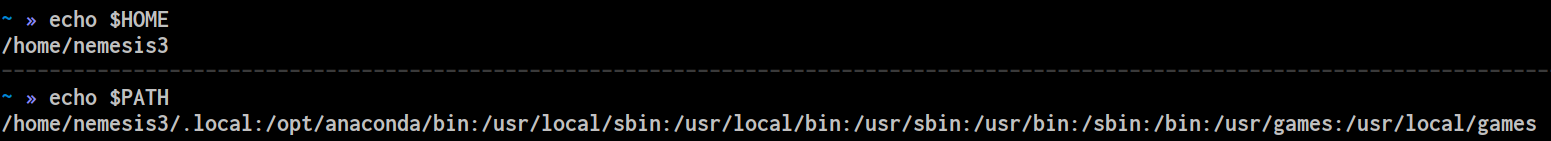
\includegraphics[width=1.00\textwidth]{pics/environment.png}
    \end{center}

    \sidebyside{0.50}{
      Script arguments are variables:
      \begin{itemize}
        \item \code{\$0}: script name
        \item \code{\$1-...}: arguments
        \item \code{\$@}: all arguments
        \item \code{\$\#}: argument number\\
          (+1, \code{\$0} counts)
      \end{itemize}
    }{\hfill}{0.43}{
      \begin{center}
        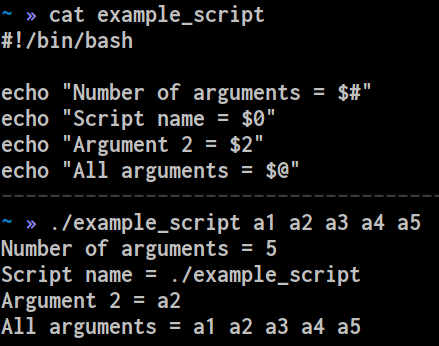
\includegraphics[width=0.90\textwidth]{pics/arguments.png}
      \end{center}
    }
  \end{center}
\end{frame}


\begin{frame}
  \begin{center}
    \frametitle{Conditionals I}

    \focus{Basic structure:}
    \code{if <test> ; then <action 1> ; else <action 2> ; fi}

    \vspace{2mm}

    \focus{Several types of conditions} can be tested,\\
    slightly different syntax

    \vspace{2mm}

    \sidebyside{0.48}{
      \centering
      First type of condition:\\
      \focus{test command output}

      \vspace{3mm}
  
      Write command in condition\\
      without parentheses

      \vspace{3mm}
  
      If return code $= 0$\\
      (usually, success)\\
      triggers \code{then},\\
      \code{else} otherwise
    }{\hfill}{0.47}{
      \begin{center}
        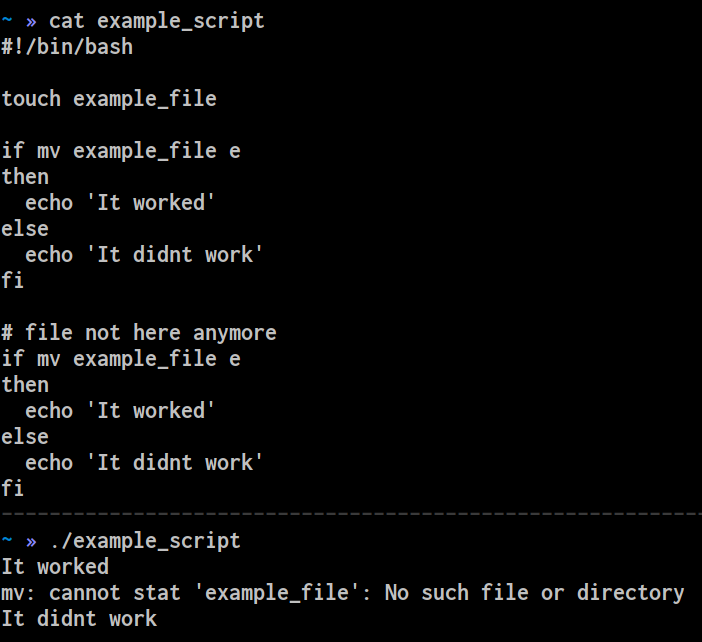
\includegraphics[width=1.00\textwidth]{pics/conditional_1.png}
      \end{center}
    }
  \end{center}
\end{frame}


\begin{frame}
  \begin{center}
    \frametitle{Conditionals II}

    \sidebyside{0.58}{
      \centering
      Second type of condition:\\
      \focus{primary expressions}

      \vspace{2mm}

      \begin{itemize}
        \item \code{[ -f <file> ]}: file exists\\
        \item \code{[ -d <directory> ]}: dir exists\\
        \item \code{[<string1> ==/!= <string2>]}
        \item \code{[<int1> <operator> <int2>]}

        \vspace{1mm}

        \code{<operator>} can be:
        \begin{itemize}
          \item \code{-eq/ne}: equal/not equal
          \item \code{-lt/le}: less/less or equal
          \item \code{-gt/ge}: greater/greater or equal
        \end{itemize}
      \end{itemize}

      \focus{Conditions within} \code{[...]}\\
      \code{[... -a ...]} is AND,\\
      \code{[... -o ...]} is OR,\\
      \code{[! ...]} is NOT
    }{\hfill}{0.40}{
      \begin{center}
        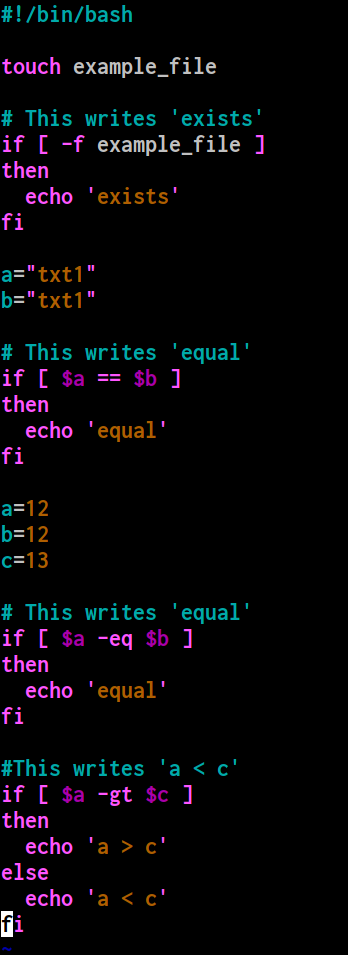
\includegraphics[width=0.68\textwidth]{pics/conditional_2.png}
      \end{center}
    }
  \end{center}
\end{frame}


\begin{frame}
  \begin{center}
    \frametitle{Iteration and loops}

    \focus{Perform actions several times}:
    \code{for <variable> in <range> ; do <action> ; done}

    \sidebyside{0.50}{
      \centering
      \code{<variable>} usually\\
      created on the spot

      \vspace{5mm}

      \code{<range>} can be:
      \begin{itemize}
        \item A given sequence (no commas)\\
        \item Matches to a regexp
      \end{itemize}

      \vspace{5mm}

      \code{<action>} can use \code{<variable>}

      \vspace{5mm}

      \focus{Example}:\\
      cycle over command-line arguments:\\
      \code{for arg in "\$@" ; ...}
    }{\hfill}{0.45}{
      \begin{center}
        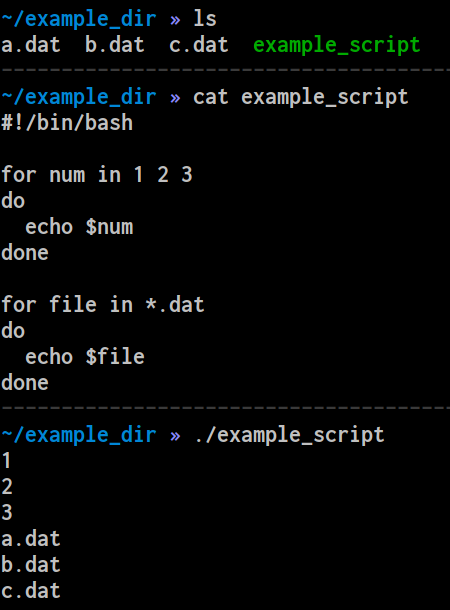
\includegraphics[width=1.00\textwidth]{pics/for.png}
      \end{center}
    }
  \end{center}
\end{frame}

\begin{frame}
	\begin{center}
		\frametitle{Exercise: file processing}

		This will be a long exercise:\\
		\focus{complex programs are done in steps}\\
		(start simple, then add complexity)

		\vspace{3mm}
	
		We have an external program, \code{binaver}, to average a column of a file:\\
		\code{binaver -r<rows> -c<columns> -k<column to average> <file>}\\
		Requires information about the files, only accepts one at a time

		\vspace{3mm}

		We will write a script (\focus{wrapper}) which:

		\begin{itemize}
			\item Counts automatically rows and columns
			\item Excludes commented lines
			\item Checks the integrity of the file
			\item Applies \code{binaver} to multiple files
		\end{itemize}
	\end{center}
\end{frame}

\begin{frame}
	\begin{center}
		\frametitle{Step I: counting rows}

		Rows can be counted with the \code{wc -l <file>} command:\\
		the command however outputs \code{<line number> <file>}

		\vspace{8mm}

		\focus{Task 1}:\\
		Write a script which assigns to a variable only the row number of a file\\
		(hint: use command substitution and a pipeline with \code{awk} or \code{cut})

		Assume the file to be the first command line argument\\
		(remember how you access it)
	\end{center}
\end{frame}

\begin{frame}
	\begin{center}
		\frametitle{Step II: counting columns}

		\focus{Task 2}:\\
		Extend the previous script, assigning to a variable\\
		the number of columns of the same file\\
		(hint: one way uses \code{awk}, its internal variables, and \code{sort})\\
		For now, assume that all rows have the same number of columns

		\vspace{8mm}

		\focus{Task 3}:\\
		Modify the script so that it proceeds only if all rows\\
		have the same number of columns\\
		(hint: if you did it as suggested before,\\
		you could use the previous bit of the script here)\\
		This checks the \focus{integrity} of the file

	\end{center}
\end{frame}


\begin{frame}
	\begin{center}
		\frametitle{Step III: comments and finalization}

		\focus{Task 4}:\\
		Modify all parts of the previous script to exclude commented lines\\
		(starting with \code{\#})\\
		(hint: you can use \code{grep})

		\vspace{4mm}

		\focus{Task 5}:\\
		Ask the user which column he wants to perform the average on\\
		(hint: \code{read -p})

		\vspace{4mm}

		\focus{Task 6}:\\
		Complete the script, applying \code{binaver} to \code{\$1} with the known info
	\end{center}
\end{frame}


\begin{frame}
	\begin{center}
		\frametitle{Step IV: robustness, multiple files}

		\focus{Task 7}:\\
		Extend the script to accept multiple files and act on all of them\\
		(hint: loop over arguments, \code{binaver} takes one at a time)

		\vspace{8mm}

		\focus{Task 8}:\\
		Increase robustness: skip a file if it doesn't exist\\
		(hint: use conditionals, the \code{else} branch can be empty)

		\vspace{8mm}

    \focus{We're done!}
	\end{center}
\end{frame}


\begin{frame}
	\begin{center}
		\frametitle{Final Notes}

    A few pieces of advice:

    \vspace{6mm}

    \begin{itemize}
      \item Sometimes it's worth settling for the easy and tedious solution.
        However, try to check out if you can do things in a smarter way\\
        and \focus{work less (!!!)}

      \vspace{4mm}

      \item You will remember the details in time. For now, \focus{rough is enough}:\\
        ``\textit{I can do this with \code{tail}, but I don't remember the options}''\\
        is ok, if you have internet access

      \vspace{4mm}

      \item Give \code{vim}/\code{emacs} and the shell a shot, it will pay you
        back tenfold
    \end{itemize}

    \vspace{6mm}

    Good luck out there!
	\end{center}
\end{frame}


\end{document}
